\documentclass[12pt,a4paper,oneside]{book}

% Universal Encoding & Packages (Compiles cleanly across pdfLaTeX, XeLaTeX, and LuaLaTeX)
\usepackage{float}
\usepackage[utf8]{inputenc}
\usepackage[T1]{fontenc}
\usepackage{lmodern}
\usepackage[a4paper, margin=1in]{geometry}

\usepackage{graphicx}
\usepackage{amsmath,amssymb}
\usepackage{hyperref}
\usepackage{xcolor}
\usepackage{listings}
\usepackage{microtype}
\usepackage{booktabs}
\usepackage{tabularx}
\usepackage{tikz}
\usetikzlibrary{shapes.geometric, arrows.meta, positioning, fit, backgrounds, shapes.multipart}

% Code Listing Configuration
\lstset{
    language=C++,
    basicstyle=\ttfamily\small,
    keywordstyle=\color{blue}\bfseries,
    stringstyle=\color{red!80!black},
    commentstyle=\color{green!60!black}\itshape,
    numbers=left,
    numberstyle=\tiny\color{gray},
    stepnumber=1,
    numbersep=8pt,
    backgroundcolor=\color{gray!5},
    showstringspaces=false,
    breaklines=true,
    frame=single,
    tabsize=4,
    captionpos=b
}

\makeatletter
\newcommand{\chapterauthor}[1]{%
  {\parindent0pt\vspace*{-15pt}%
  \linespread{1.1}\large\itshape\begin{flushright}#1\end{flushright}%
  \par\nobreak\vspace*{25pt}}
  \@afterheading%
}
\makeatother

\begin{document}

\mainmatter

% Set Chapter counter to 4 so the upcoming \chapter automatically becomes Chapter 5
\setcounter{chapter}{4}

\chapter{C++ WebAssembly Sudoku Solver \& Game System}
\chapterauthor{Akash Prajapati(251103), Swaraj Koushik(251105)}

% =====================================================================
% Section 5.1: Introduction and Problem Statement
% =====================================================================
\section{Introduction and Problem Statement}
Sudoku is a logic-based combinatorial puzzle that requires filling a $9 \times 9$ grid with digits from 1 through 9 such that every row, column, and $3 \times 3$ subgrid contains each digit exactly once without duplication. While the game rules are straightforward for human players, solving difficult puzzles algorithmically is an established NP-complete problem. 

When implemented entirely in client-side interpreted JavaScript, recursive algorithms such as depth-first search (DFS) backtracking often suffer from noticeable execution latency, high memory usage, and call-stack limits on low-power devices. Conversely, native C++ desktop applications provide lightning-fast solving performance, but they require users to compile, install, and manage platform-specific software.

To solve this dilemma, we designed our project around a decoupled, two-tier architecture. All core domain logic, grid representation, coordinate uniqueness checking, and recursive backtracking routines are implemented in modern C++ (C++17) using clean Object-Oriented principles. Using the Emscripten toolchain, we compile the C++ backend into portable WebAssembly (Wasm). This allows the solver to run directly inside any modern web browser at near-native speeds (consistently solving in under 5 milliseconds) with zero server infrastructure required. A lightweight frontend built with HTML5, CSS Grid, and vanilla JavaScript provides an interactive, responsive user experience complete with a live stopwatch, an on-screen phone keypad, rough candidate notes, and multi-theme personalization.

% =====================================================================
% Section 5.2: Scope and Feature Set
% =====================================================================
\section{Scope and Feature Set}
The application delivers a comprehensive suite of gameplay, algorithmic, and interface features:
\begin{itemize}
    \item \textbf{High-Speed C++ Backtracking Engine:} Implements recursive depth-first search with constraint-based pruning to solve valid $9 \times 9$ boards in under 5 milliseconds directly in the browser.
    \item \textbf{Dynamic Multi-Tier Puzzle Generation:} Uses randomized board generation and difficulty-parameterized clue carving to synthesize puzzles on demand across Easy (41 clues), Medium (31 clues), and Hard (21 clues) tiers.
    \item \textbf{Smart Hint System:} Evaluates the player's board in real time, solves it in the background via C++ WebAssembly, and reveals a single verified number either at the player's actively selected square or across a randomly chosen empty cell without exposing the rest of the board.
    \item \textbf{On-Screen 3x3 Phone Keypad:} Features a dedicated numeric keypad arranged in a 3x3 phone layout (digits 1--9) placed conveniently to the right of the board for mouse and touchscreen gameplay.
    \item \textbf{3x3 Rough Candidate Notes (Pencil Mode):} Each cell contains an embedded 3x3 mini-grid. Toggling Notes Mode allows players to jot down, toggle, and erase 1--9 candidate possibilities before committing to an entry.
    \item \textbf{Dynamic Crosshair \& Duplicate Highlighting:} Selecting any square illuminates its entire row, column, and $3 \times 3$ subgrid, while simultaneously highlighting all identical numbers across the board for rapid visual scanning.
    \item \textbf{Real-Time Conflict Detection \& Per-Cell Red Highlighting:} Live mathematical validation checks for duplicate digits across rows, columns, and 3x3 boxes on every entry. Conflicting cells immediately illuminate in bright red, the board border glows red, and a shake animation triggers.
    \item \textbf{Player-Only Victory Recognition:} Differentiates between human player completion and automated solving via the C++ engine. The victory celebration and completion timer trigger strictly when the human player finishes the board.
    \item \textbf{Question Cell Cursor Protection:} Starting clues are permanently marked read-only and styled with default arrow cursors, preventing caret blinking or hand pointers on immutable numbers.
    \item \textbf{Multi-Theme Customization:} Features a responsive background theme picker supporting seven distinct palettes: Ocean, Wood, Sky, Space, Nature, Dark Slate, and Clean Light.
    \item \textbf{Live Game Timer:} An integrated stopwatch tracks elapsed solving time with play/pause controls.
\end{itemize}

% =====================================================================
% Section 5.3: Tools and Technology Stack
% =====================================================================
\section{Tools and Technology Stack}
To build and deploy a decoupled WebAssembly application, we selected a toolchain that bridges low-level systems programming with high-level browser technologies. Modern C++17 provides strict type safety, predictable memory management, and efficient recursive algorithms. Emscripten acts as the critical bridge, compiling the C++ source files into compact WebAssembly bytecode while generating the JavaScript runtime glue. The frontend relies exclusively on standard web technologies without heavy external frameworks, keeping load times minimal.

Table~\ref{tab:tools} summarizes the complete development environment and the specific role of each technology.

\begin{table}[htbp]
\centering
\begin{tabularx}{\textwidth}{l p{4.2cm} X}
\toprule
\textbf{Category} & \textbf{Tool / Technology} & \textbf{Role in System} \\
\midrule
Language & Modern C++ (C++17) & Implements atomic domain models, 3x3 constraint algorithms, and recursive backtracking. \\
Compiler & Emscripten SDK (\texttt{emsdk}) & Compiles C++ source into portable WebAssembly bytecode (\texttt{solver.wasm}) and JS glue (\texttt{solver.js}). \\
Frontend & HTML5, CSS Grid, ES6+ & Provides responsive layout, 3x3 candidate subgrids, theme stylesheets, and touch/keyboard controls. \\
Local Server & Python \texttt{http.server} & Serves WebAssembly binaries with compliant MIME types, bypassing local browser CORS blocks. \\
Typesetting & LaTeX \& TikZ & Typesets academic documentation and renders native vector UML and flow diagrams. \\
Version Control & Git \& GitHub & Manages project versioning, feature branches, and collaboration history. \\
\bottomrule
\end{tabularx}
\caption{Technology stack and development toolchain.}
\label{tab:tools}
\end{table}

% =====================================================================
% Section 5.4: Object-Oriented Architecture
% =====================================================================
\section{Object-Oriented Architecture}
The system is built upon foundational Object-Oriented Programming (OOP) paradigms to ensure modularity, separation of concerns, and future extensibility.

\subsection{Class Design and Associations}
The C++ domain architecture consists of four primary entities:
\begin{itemize}
    \item \textbf{Encapsulation (\texttt{Cell} and \texttt{Board}):} The \texttt{Cell} class encapsulates its internal digit (strictly constrained to $0 \le \text{val} \le 9$) and its fixed-state boolean flag. The \texttt{Board} class encapsulates the 81-cell matrix (\texttt{Cell grid[9][9]}). Direct member modifications are prevented; callers must invoke \texttt{board.setCell()}, which enforces domain boundary invariants and protects given clues.
    \item \textbf{Abstraction \& Strategy Pattern (\texttt{SudokuSolver}):} To decouple board representation from solving algorithms, we declared an abstract base class \texttt{SudokuSolver} with a pure virtual contract \texttt{virtual bool solve(Board\& board) = 0}. Concrete strategies (\texttt{BacktrackingSolver} and \texttt{RandomGenerator}) inherit from this interface, allowing algorithmic strategies to be swapped without modifying the board or UI.
\end{itemize}

Figure~\ref{fig:uml_class} illustrates the class hierarchy, member attributes, methods, and access specifiers.

\begin{figure}[htbp]
\centering
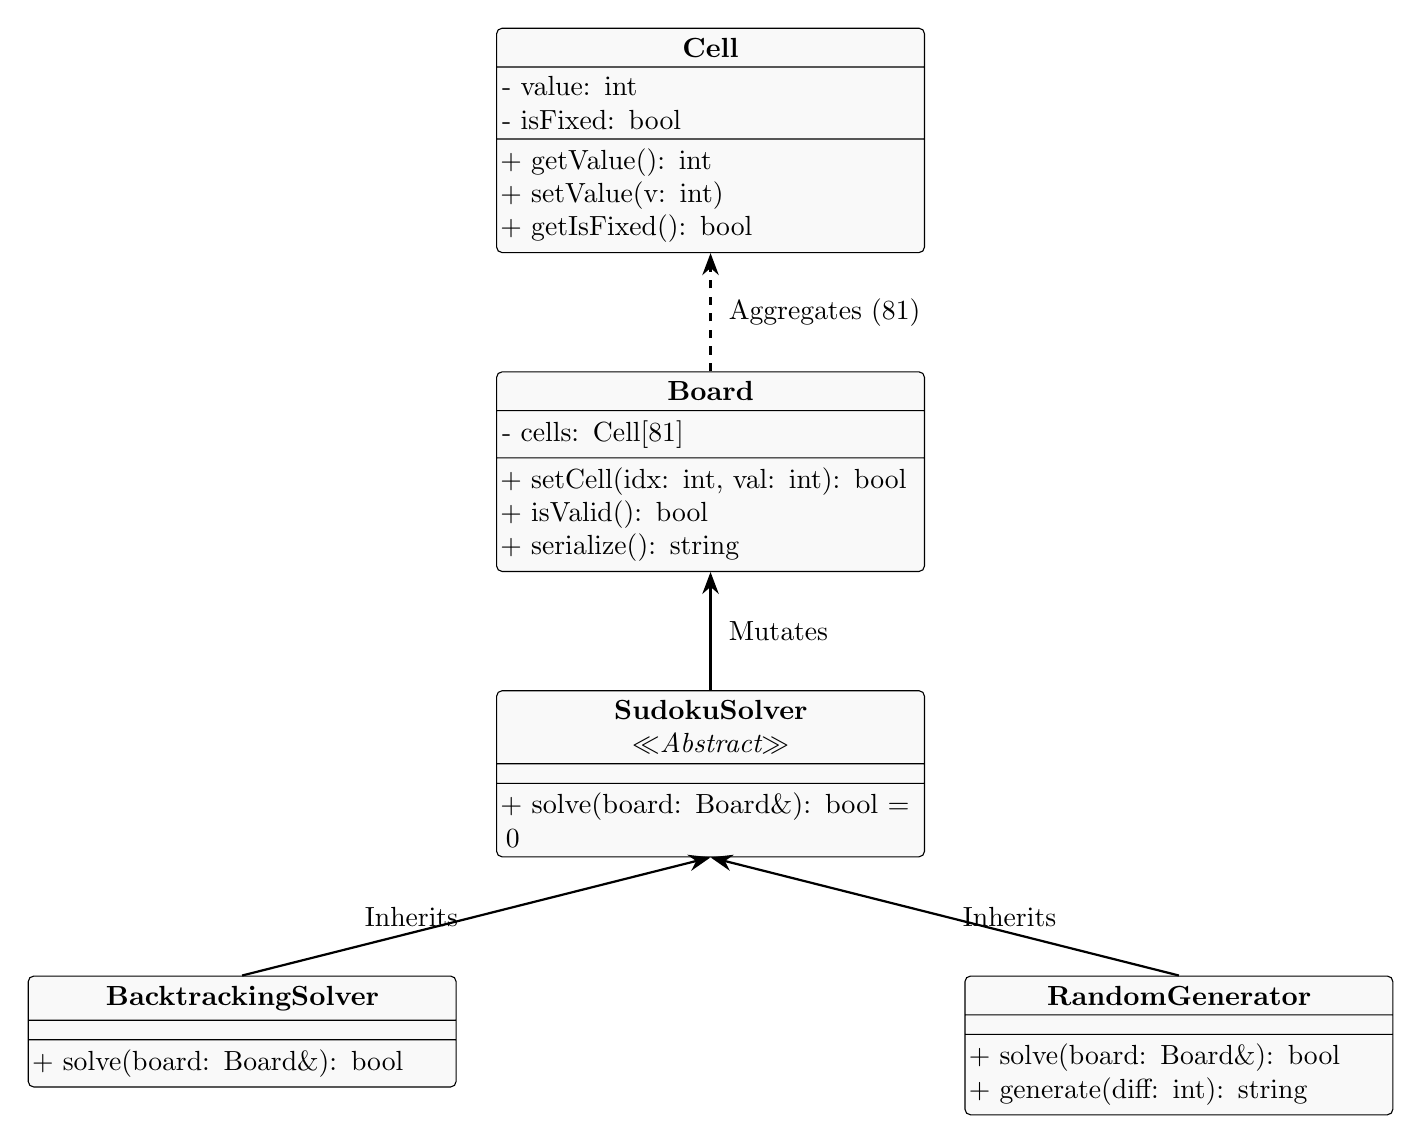
\begin{tikzpicture}[
    node distance=1.5cm and 2cm,
    umlclass/.style={draw, rectangle split, rectangle split parts=3, 
                     fill=gray!5, text width=5.2cm, 
                     rounded corners=2pt,
                     every text node part/.style={align=center},
                     every second node part/.style={align=left},
                     every third node part/.style={align=left}},
    arrow/.style={-{Stealth[scale=1.2]}, thick},
    dashedarrow/.style={-{Stealth[scale=1.2]}, dashed, thick}
]

% Nodes
\node[umlclass] (Solver) {
    \textbf{SudokuSolver} \\ \textit{$\ll$Abstract$\gg$}
    \nodepart{second}
    \nodepart{third}
    + solve(board: Board\&): bool = 0
};
\node[umlclass, below left=1.5cm and 0.5cm of Solver] (Backtrack) {
    \textbf{BacktrackingSolver}
    \nodepart{second}
    \nodepart{third}
    + solve(board: Board\&): bool
};
\node[umlclass, below right=1.5cm and 0.5cm of Solver] (Generator) {
    \textbf{RandomGenerator}
    \nodepart{second}
    \nodepart{third}
    + solve(board: Board\&): bool \\
    + generate(diff: int): string
};
\node[umlclass, above=1.5cm of Solver] (Board) {
    \textbf{Board}
    \nodepart{second}
    - cells: Cell[81]
    \nodepart{third}
    + setCell(idx: int, val: int): bool \\
    + isValid(): bool \\
    + serialize(): string
};
\node[umlclass, above=1.5cm of Board] (Cell) {
    \textbf{Cell}
    \nodepart{second}
    - value: int \\
    - isFixed: bool
    \nodepart{third}
    + getValue(): int \\
    + setValue(v: int) \\
    + getIsFixed(): bool
};

% Relationships
\draw[arrow] (Backtrack.north) -- (Solver.south) node[midway, left=0.1cm] {Inherits};
\draw[arrow] (Generator.north) -- (Solver.south) node[midway, right=0.1cm] {Inherits};
\draw[arrow] (Solver.north) -- (Board.south) node[midway, right=0.1cm] {Mutates};
\draw[dashedarrow] (Board.north) -- (Cell.south) node[midway, right=0.1cm] {Aggregates (81)};

\end{tikzpicture}
\caption{UML Class Diagram illustrating structural relationships and inheritance hierarchy.}
\label{fig:uml_class}
\end{figure}

\subsection{Code Snippet: Abstraction \& Encapsulation}
The C++ implementation below illustrates how encapsulation and abstract polymorphism work together:

\begin{lstlisting}
class Board {
private:
    Cell grid[81]; // Encapsulated matrix
public:
    bool setCell(int index, int value) {
        if (!grid[index].isFixed()) {
            grid[index].setValue(value);
            return true;
        }
        return false;
    }
};

// Abstract Strategy Interface
class SudokuSolver {
public:
    virtual bool solve(Board& board) = 0; // Pure virtual function
    virtual ~SudokuSolver() {}
};

class BacktrackingSolver : public SudokuSolver {
public:
    bool solve(Board& board) override {
        // Recursive depth-first search with pruning
    }
};
\end{lstlisting}

% =====================================================================
% Section 5.5: System Architecture & Flow Diagrams
% =====================================================================
\section{System Architecture \& Flow Diagrams}
To thoroughly document how the software is structured and how it behaves dynamically at runtime, we modeled the application across three complementary architectural views: high-level component tiering, operational control sequencing, and cross-runtime data pipelining.

\subsection{System Architecture Diagram}
Figure~\ref{fig:architecture} illustrates the decoupled two-tier architecture. The frontend tier operates completely within the client browser sandbox, managing the DOM grid, on-screen keypad inputs, and active UI states. When solving or hint operations are triggered, the WebAssembly boundary coordinates data exchange using stateless 81-character string serialization. The backend C++ tier receives the serialized payload, reconstructs the object graph, executes recursive backtracking, and serializes the resolved grid back to the DOM without incurring cross-runtime memory leaks.

\begin{figure}[htbp]
\centering
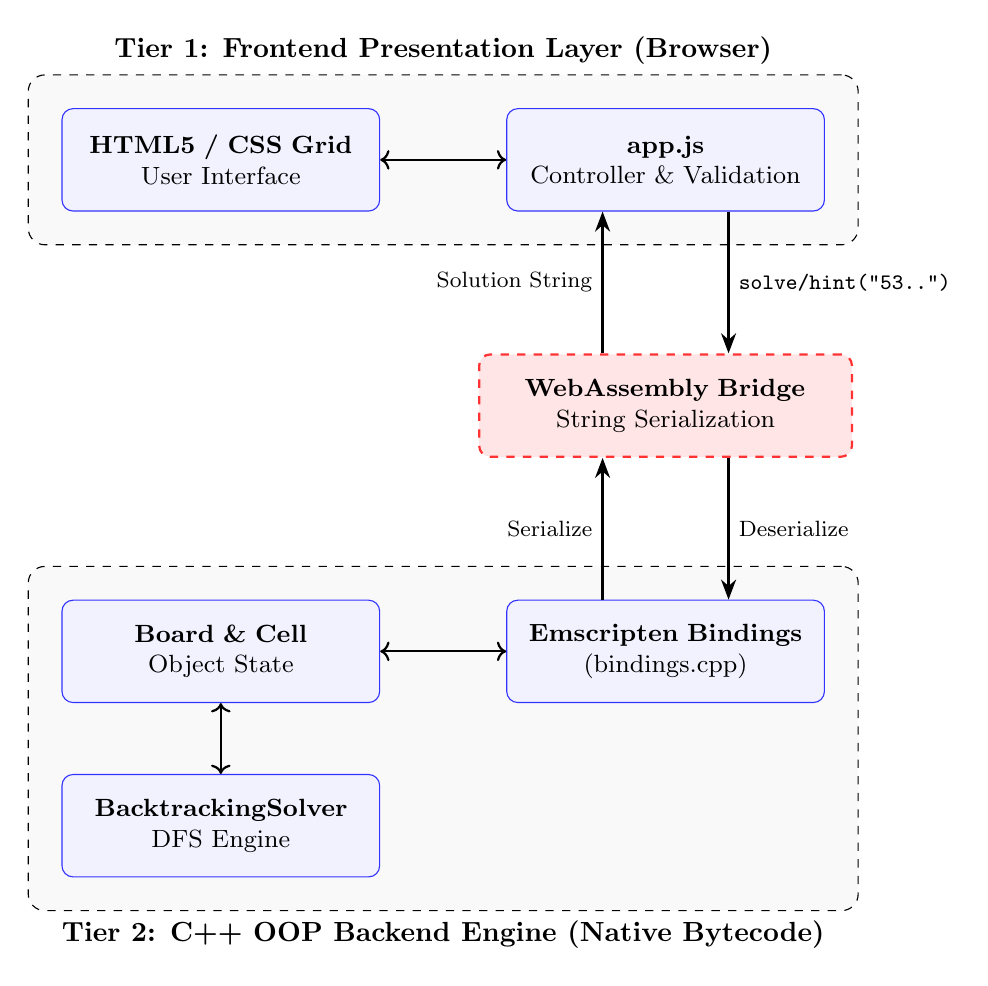
\begin{tikzpicture}[
    node distance=1.5cm and 1cm,
    block/.style={rectangle, draw=blue!80, fill=blue!5, text width=3.8cm, text centered, minimum height=1.3cm, rounded corners=4pt, font=\small},
    wblock/.style={rectangle, draw=red!80, fill=red!10, text width=4.5cm, text centered, minimum height=1.3cm, rounded corners=4pt, dashed, thick, font=\small},
    arrow/.style={-{Stealth[scale=1.1]}, thick},
    container/.style={rectangle, draw, dashed, fill=gray!5, inner sep=12pt, rounded corners=6pt}
]

% Row 1: Frontend
\node[block] (UI) {\textbf{HTML5 / CSS Grid} \\ User Interface};
\node[block, right=1.6cm of UI] (JS) {\textbf{app.js} \\ Controller \& Validation};
\draw[<->, thick] (UI) -- (JS);

\begin{scope}[on background layer]
    \node[container, fit=(UI) (JS), label=above:\textbf{Tier 1: Frontend Presentation Layer (Browser)}] (Front) {};
\end{scope}

% Row 2: Boundary
\node[wblock, below=1.8cm of JS] (Wasm) {\textbf{WebAssembly Bridge} \\ String Serialization};

\draw[arrow] ([xshift=0.8cm]JS.south) -- ([xshift=0.8cm]Wasm.north) node[midway, right, font=\footnotesize] {\texttt{solve/hint("53..")}};
\draw[arrow] ([xshift=-0.8cm]Wasm.north) -- ([xshift=-0.8cm]JS.south) node[midway, left, font=\footnotesize] {Solution String};

% Row 3: Backend
\node[block, below=1.8cm of Wasm] (API) {\textbf{Emscripten Bindings} \\ (bindings.cpp)};
\node[block, left=1.6cm of API] (Board) {\textbf{Board \& Cell} \\ Object State};
\node[block, below=0.9cm of Board] (Solver) {\textbf{BacktrackingSolver} \\ DFS Engine};

\draw[arrow] ([xshift=0.8cm]Wasm.south) -- ([xshift=0.8cm]API.north) node[midway, right, font=\footnotesize] {Deserialize};
\draw[arrow] ([xshift=-0.8cm]API.north) -- ([xshift=-0.8cm]Wasm.south) node[midway, left, font=\footnotesize] {Serialize};

\draw[<->, thick] (API) -- (Board);
\draw[<->, thick] (Board) -- (Solver);

\begin{scope}[on background layer]
    \node[container, fit=(API) (Board) (Solver), label=below:\textbf{Tier 2: C++ OOP Backend Engine (Native Bytecode)}] (Back) {};
\end{scope}

\end{tikzpicture}
\caption{System Architecture Diagram illustrating the decoupled two-tier WebAssembly design.}
\label{fig:architecture}
\end{figure}

\subsection{Control Flow Diagram (CFD)}
Figure~\ref{fig:cfd} illustrates the complete execution pipeline triggered when a user enters an input, clicks the keypad, or toggles candidate notes. The system validates cell immutability, checks the active mode, updates board state, computes conflict indices, and checks victory status.

\begin{figure}[htbp]
\centering
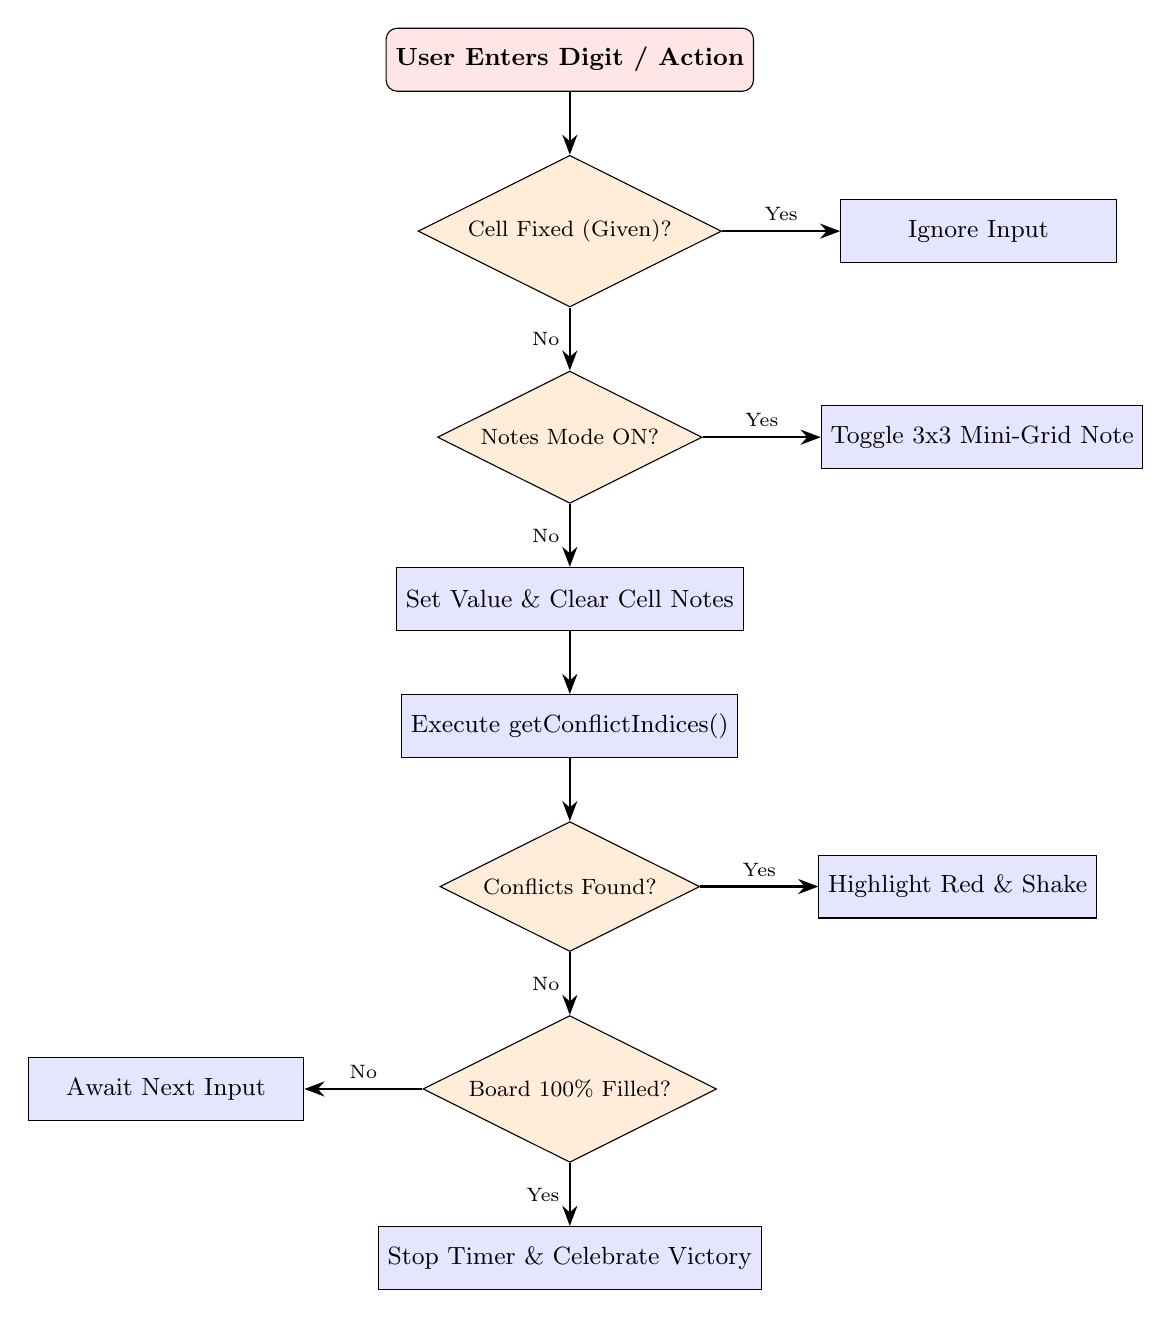
\begin{tikzpicture}[
    node distance=1.2cm and 1.5cm,
    startstop/.style={rectangle, rounded corners, minimum width=3cm, minimum height=0.8cm, text centered, draw=black, fill=red!10, font=\small\bfseries},
    process/.style={rectangle, minimum width=3.5cm, minimum height=0.8cm, text centered, draw=black, fill=blue!10, font=\small},
    decision/.style={diamond, aspect=2, minimum width=3.2cm, minimum height=0.8cm, text centered, draw=black, fill=orange!15, font=\footnotesize},
    arrow/.style={thick, -{Stealth[scale=1.1]}}
]

\node[startstop] (start) {User Enters Digit / Action};
\node[decision, below=0.8cm of start] (dec1) {Cell Fixed (Given)?};
\node[process, right=1.5cm of dec1] (ignore) {Ignore Input};
\node[decision, below=0.8cm of dec1] (dec2) {Notes Mode ON?};
\node[process, right=1.5cm of dec2] (notes) {Toggle 3x3 Mini-Grid Note};
\node[process, below=0.8cm of dec2] (place) {Set Value \& Clear Cell Notes};
\node[process, below=0.8cm of place] (validate) {Execute getConflictIndices()};
\node[decision, below=0.8cm of validate] (dec3) {Conflicts Found?};
\node[process, right=1.5cm of dec3] (error) {Highlight Red \& Shake};
\node[decision, below=0.8cm of dec3] (dec4) {Board 100\% Filled?};
\node[process, below=0.8cm of dec4] (win) {Stop Timer \& Celebrate Victory};
\node[process, left=1.5cm of dec4] (continue) {Await Next Input};

\draw[arrow] (start) -- (dec1);
\draw[arrow] (dec1) -- node[above, font=\scriptsize] {Yes} (ignore);
\draw[arrow] (dec1) -- node[left, font=\scriptsize] {No} (dec2);
\draw[arrow] (dec2) -- node[above, font=\scriptsize] {Yes} (notes);
\draw[arrow] (dec2) -- node[left, font=\scriptsize] {No} (place);
\draw[arrow] (place) -- (validate);
\draw[arrow] (validate) -- (dec3);
\draw[arrow] (dec3) -- node[above, font=\scriptsize] {Yes} (error);
\draw[arrow] (dec3) -- node[left, font=\scriptsize] {No} (dec4);
\draw[arrow] (dec4) -- node[left, font=\scriptsize] {Yes} (win);
\draw[arrow] (dec4) -- node[above, font=\scriptsize] {No} (continue);

\end{tikzpicture}
\caption{Control Flow Diagram (CFD) of user input, candidate notes, and conflict checking.}
\label{fig:cfd}
\end{figure}

\subsection{Data Flow Diagram (DFD)}
Figure~\ref{fig:dfd} traces how state data moves between the player interface, memory stores, and the compiled WebAssembly routines. Data paths are cleanly partitioned with dedicated parallel channels and offset routing to prevent visual overlap.

\begin{figure}[htbp]
\centering
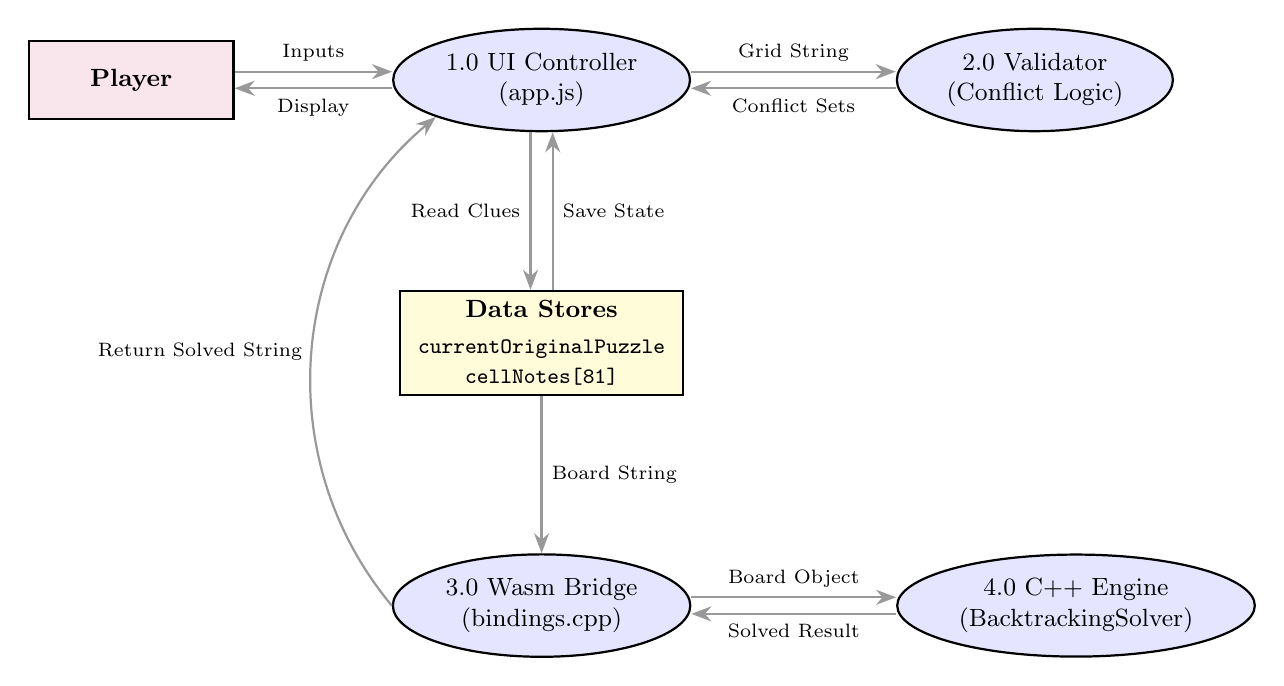
\begin{tikzpicture}[
    node distance=1.6cm and 2.4cm,
    entity/.style={rectangle, draw=black, thick, fill=purple!10, minimum width=2.6cm, minimum height=1.0cm, align=center, font=\small\bfseries},
    process/.style={ellipse, draw=black, thick, fill=blue!10, minimum width=3.4cm, minimum height=1.2cm, align=center, font=\small},
    storage/.style={rectangle, draw=black, thick, fill=yellow!15, minimum width=3.6cm, minimum height=1.1cm, align=center, font=\small},
    flow/.style={thick, -{Stealth[scale=1.1]}, draw=gray!80}
]

\node[entity] (user) {Player};
\node[process, right=2.0cm of user] (p1) {1.0 UI Controller\\(app.js)};
\node[process, right=2.6cm of p1] (p2) {2.0 Validator\\(Conflict Logic)};

\node[storage, below=2.0cm of p1] (d1) {\textbf{Data Stores}\\[2pt]\footnotesize\texttt{currentOriginalPuzzle}\\\footnotesize\texttt{cellNotes[81]}};

\node[process, below=2.0cm of d1] (p3) {3.0 Wasm Bridge\\(bindings.cpp)};
\node[process, right=2.6cm of p3] (p4) {4.0 C++ Engine\\(BacktrackingSolver)};

% User <-> P1
\draw[flow] ([yshift=3pt]user.east) -- node[above, font=\scriptsize] {Inputs} ([yshift=3pt]p1.west);
\draw[flow] ([yshift=-3pt]p1.west) -- node[below, font=\scriptsize] {Display} ([yshift=-3pt]user.east);

% P1 <-> P2
\draw[flow] ([yshift=3pt]p1.east) -- node[above, font=\scriptsize] {Grid String} ([yshift=3pt]p2.west);
\draw[flow] ([yshift=-3pt]p2.west) -- node[below, font=\scriptsize] {Conflict Sets} ([yshift=-3pt]p1.east);

% P1 <-> D1
\draw[flow] ([xshift=-4pt]p1.south) -- node[left, font=\scriptsize] {Read Clues} ([xshift=-4pt]d1.north);
\draw[flow] ([xshift=4pt]d1.north) -- node[right, font=\scriptsize] {Save State} ([xshift=4pt]p1.south);

% D1 -> P3
\draw[flow] (d1.south) -- node[right, font=\scriptsize] {Board String} (p3.north);

% P3 <-> P4
\draw[flow] ([yshift=3pt]p3.east) -- node[above, font=\scriptsize] {Board Object} ([yshift=3pt]p4.west);
\draw[flow] ([yshift=-3pt]p4.west) -- node[below, font=\scriptsize] {Solved Result} ([yshift=-3pt]p3.east);

% P3 -> P1 (Direct curved return on the outer perimeter)
\draw[flow] (p3.west) to[bend left=45] node[midway, left, font=\scriptsize] {Return Solved String} (p1.south west);

\end{tikzpicture}
\caption{Data Flow Diagram (Level 1 DFD) showing string serialization across runtime tiers.}
\label{fig:dfd}
\end{figure}

% =====================================================================
% Section 5.6: Prompt Documentation and Development Workflow
% =====================================================================
\section{Prompt Documentation and Development Workflow}
The project was engineered iteratively through conversational AI prompting, moving methodically from backend domain modeling to compiler debugging, UI/UX polish, and feature additions.

\subsection{README Implementation Phases}
\begin{enumerate}
    \item \textbf{README Phase 1: Core Domain Modeling (C++)}
    \begin{itemize}
        \item \textit{``Construct an atomic Cell class and an aggregate Board class in modern C++ with strict encapsulation. Ensure values are bounded between 0 and 9, fixed clues are protected from modification, and row, column, and 3x3 box uniqueness rules (startRow = r - r \% 3, startCol = c - c \% 3) are strictly verified.''}
        \item \textit{``Write a local CLI driver in main.cpp to validate coordinate boundaries, board loading from string representations, and console-based formatted display.''}
    \end{itemize}

    \item \textbf{README Phase 2: Solver Algorithm Engine (C++)}
    \begin{itemize}
        \item \textit{``Define an abstract SudokuSolver interface with a pure virtual solve(Board\&) method. Implement recursive BacktrackingSolver using Depth-First Search with empty-cell discovery and candidate backtracking.''}
        \item \textit{``Implement PuzzleGenerator by taking a fully solved randomized board and removing clues according to difficulty levels: 40 for Easy, 50 for Medium, and 60 for Hard. Validate execution against unsolvable edge-case puzzle states.''}
    \end{itemize}

    \item \textbf{README Phase 3: Web Presentation Layer (HTML/CSS/JS)}
    \begin{itemize}
        \item \textit{``Build a 9x9 CSS Grid layout with distinct 3x3 block borders, single-digit input filtering (1--9), and directional arrow-key navigation.''}
        \item \textit{``Design a 'Generate Puzzle' feature with an HTML dialog modal for selecting Easy, Medium, and Hard difficulties, including dark backdrop blur and modal actions.''}
    \end{itemize}

    \item \textbf{README Phase 4: Integration Bridge (WebAssembly via Emscripten)}
    \begin{itemize}
        \item \textit{``Expose C++ Board serialization and solver entry points to JavaScript using EMSCRIPTEN\_BINDINGS so that the solver executes natively in the browser without server dependencies.''}
        \item \textit{``Explain how EMSCRIPTEN\_BINDINGS operates and how the C++ to JavaScript WebAssembly bridge coordinates string serialization across the memory boundary.''}
    \end{itemize}

    \item \textbf{README Phase 5: Verification, State Management \& UI Polish}
    \begin{itemize}
        \item \textit{``Implement Phase 5 polish, including CSS shake animations for invalid/unsolvable boards, visual clue differentiation, and a clear distinction between the Reset button (restoring starting clues) and the Clear button (wiping the board).''}
        \item \textit{``Fix frontend bugs related to locking generated clues (read-only cells), fixing the reset baseline, and adding real-time conflict validation.''}
        \item \textit{``Append a styled 'How to Play' instruction card directly below the grid for intuitive onboarding.''}
    \end{itemize}
\end{enumerate}

\subsection{Toolchain \& Build Debugging Prompts}
\begin{itemize}
    \item \textbf{IntelliSense Header Discovery:} \textit{``Troubleshoot VS Code IntelliSense include errors for Emscripten bindings where <emscripten/bind.h> is flagged with red squiggles, and provide the exact c\_cpp\_properties.json configuration.''}
    \item \textbf{Compiler Driver Mismatch:} \textit{``Debug wasm-ld linking errors caused by using the emcc C compiler instead of the em++ C++ compiler when compiling and linking C++ standard library files and embind objects.''}
    \item \textbf{Local Web Server Setup:} \textit{``Clarify deployment requirements regarding the Emscripten environment script (source emsdk\_env.sh) for compilation versus running the Python HTTP server (python3 -m http.server) to bypass browser CORS restrictions on WebAssembly binaries.''}
\end{itemize}

\subsection{Feature Expansion \& Runtime Debugging Prompts}
\begin{itemize}
    \item \textbf{Smart Hint Specification \& Zero-Recompile Resolution:} \textit{``Design a Smart Hint system where JavaScript sends the current board to C++, solves it in the background, reveals a single correct number at the focused square, and highlights it on the UI. Resolve the resulting runtime error 'TypeError: sudokuModule.getSmartHint is not a function' by routing through the pre-compiled solvePuzzle endpoint.''}
    \item \textbf{Defensive Event Listener Hardening:} \textit{``Diagnose why buttons stopped responding due to uncaught null-reference TypeErrors on dynamically created elements, and implement defensive null-checks across all button event registrations.''}
    \item \textbf{Conflict Highlight Specificity Fix:} \textit{``Diagnose why conflicting duplicate cells were not turning red upon validation, and implement getConflictIndices() with high-specificity CSS rules to override active cell styling.''}
    \item \textbf{Theme Contrast Refinement:} \textit{``Darken the highlighted crosshair and same-number tint colors for Wood, Sky, and Clean Light themes to ensure strong contrast against bright cell backgrounds.''}
    \item \textbf{Player Victory Separation:} \textit{``Ensure that the completion celebration only fires when the human player finishes the board, preventing the C++ Solve button from triggering the player congratulations message.''}
\end{itemize}

% =====================================================================
% Section 5.7: Project Screenshots
% =====================================================================
\clearpage
\section{Project Screenshots}
\vspace{-0.5em}
This section presents the graphical user interface of the running Sudoku application across various visual themes, functional modes, and interactive dialogs.

\begin{figure}[H]
\centering
\vspace{-0.5em}
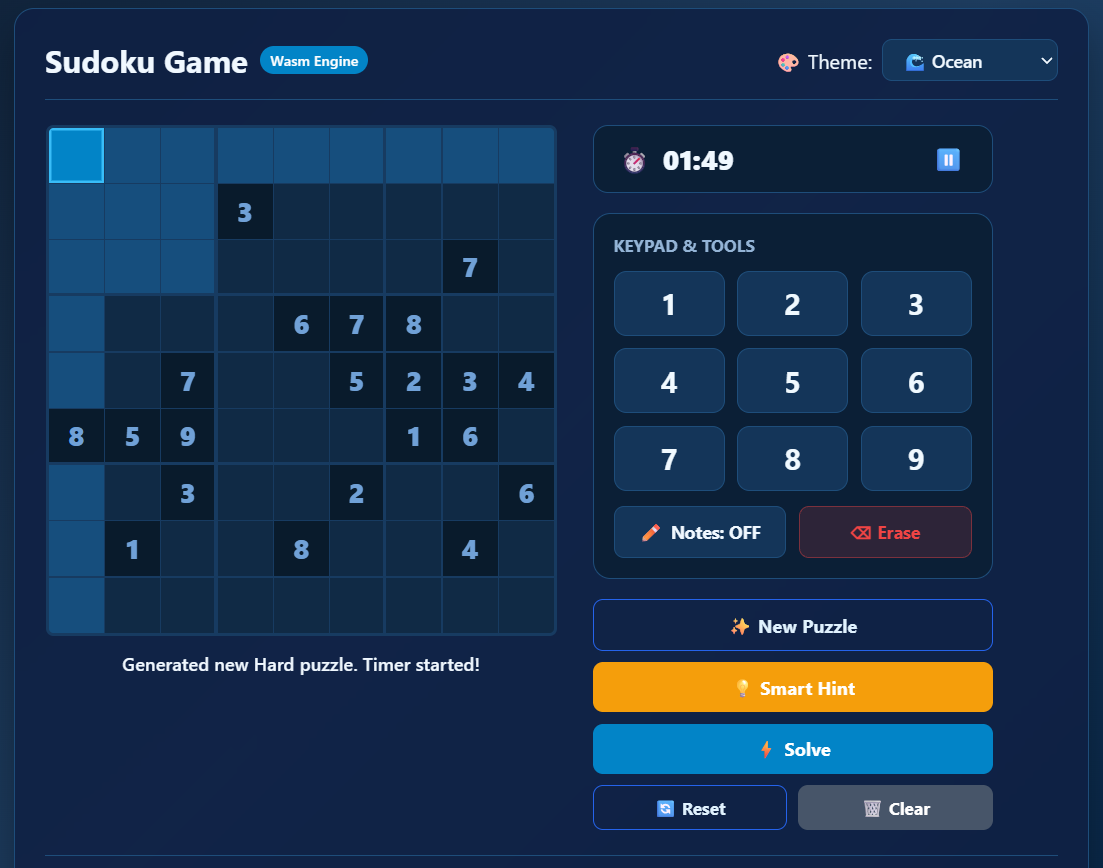
\includegraphics[width=0.62\textwidth]{S1.png}
\vspace{-0.5em}
\caption{Primary gameplay interface in Ocean theme, featuring the 9x9 board, live stopwatch, 3x3 phone keypad, and game control buttons.}
\label{fig:screenshot_s1}
\end{figure}

\begin{figure}[H]
\centering
\vspace{-0.5em}
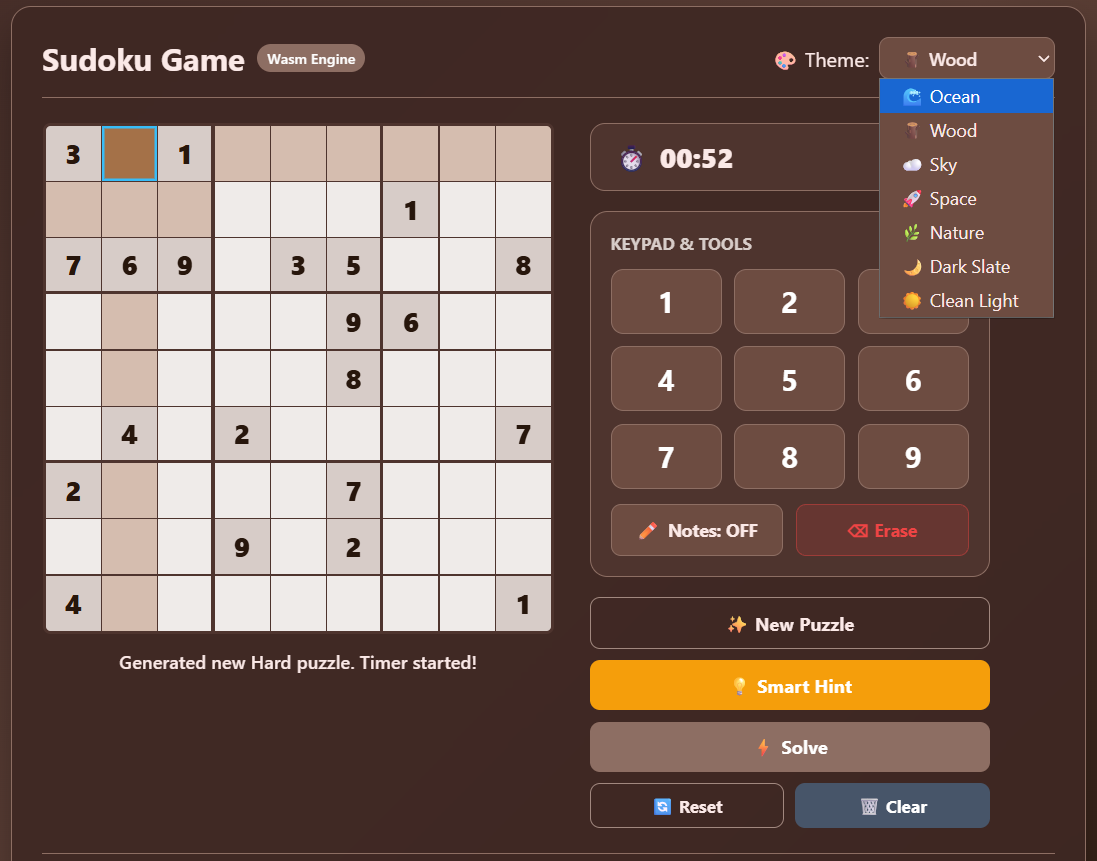
\includegraphics[width=0.62\textwidth]{S2.png}
\vspace{-0.5em}
\caption{Multi-theme customization menu in Wood theme, demonstrating real-time palette switching across seven distinct themes.}
\label{fig:screenshot_s2}
\end{figure}

\begin{figure}[H]
\centering
\vspace{-0.5em}
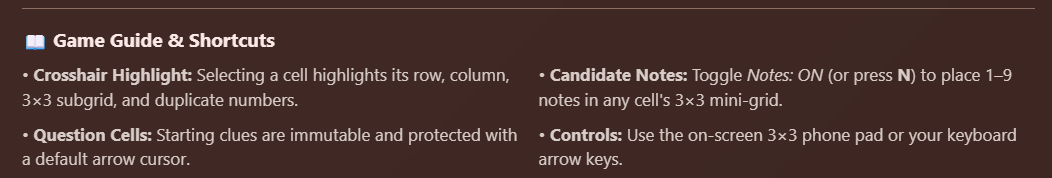
\includegraphics[width=0.68\textwidth]{S3.png}
\vspace{-0.5em}
\caption{In-game onboarding drawer illustrating game rules, candidate notes instructions, and keyboard navigation shortcuts.}
\label{fig:screenshot_s3}
\end{figure}

\clearpage
\begin{figure}[H]
\centering
\vspace{-0.5em}
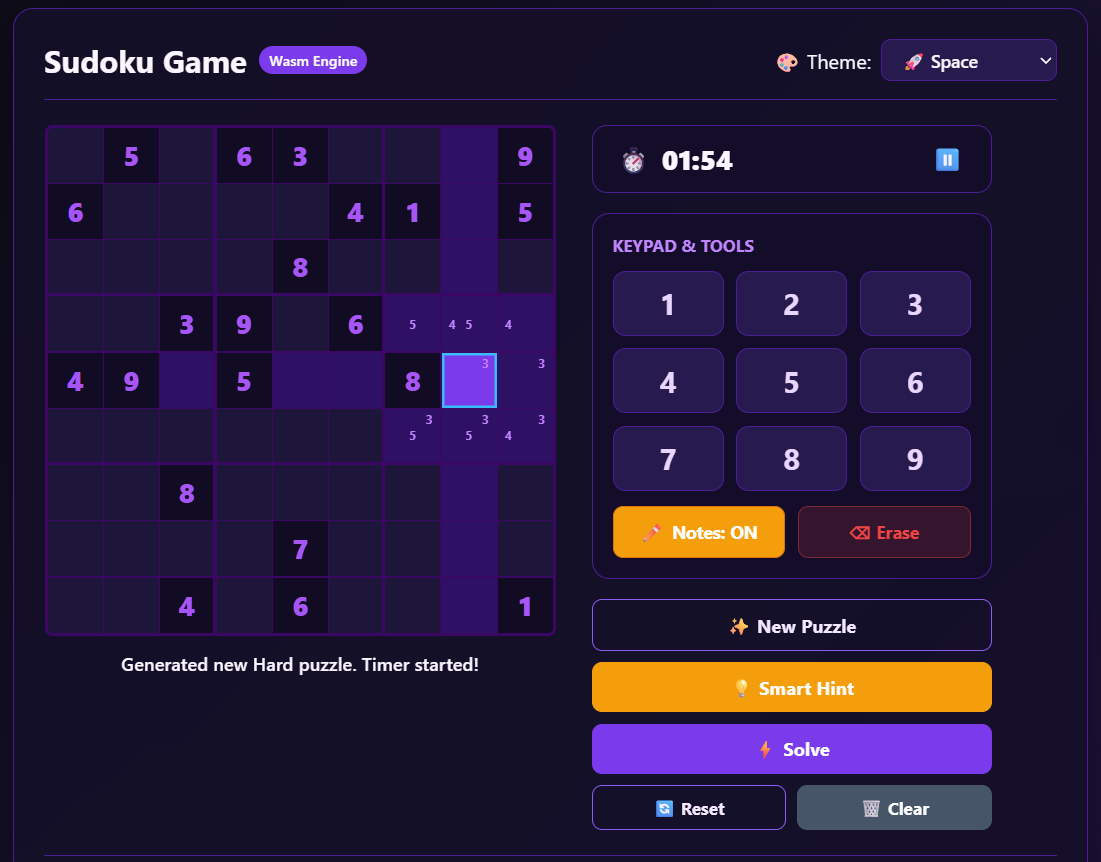
\includegraphics[width=0.62\textwidth]{S4.png}
\vspace{-0.5em}
\caption{Candidate Notes (Pencil Mode) active in Space theme, showing rough 1--9 possibilities rendered within the cell's 3x3 mini-grid.}
\label{fig:screenshot_s4}
\end{figure}

\begin{figure}[H]
\centering
\vspace{-0.5em}
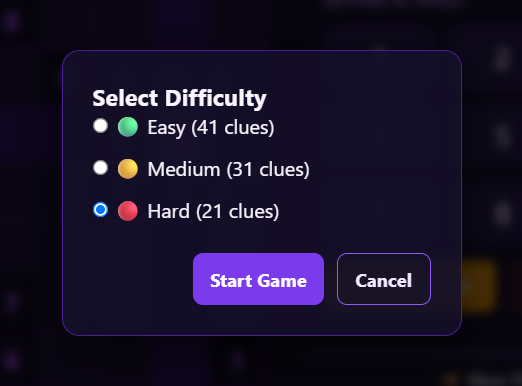
\includegraphics[width=0.48\textwidth]{S5.png}
\vspace{-0.5em}
\caption{Difficulty configuration modal dialog with backdrop blur, allowing players to select Easy (41 clues), Medium (31 clues), or Hard (21 clues).}
\label{fig:screenshot_s5}
\end{figure}

\end{document}